\chapter{Análise de velocidade de escoamento no perfil}
É necessário verificar se a velocidade máxima desenvolvida no entorno do perfil da asa em velocidade de cruzeiro não ultrapasse Mach 1. A presença de escoamento transônico sobre a asa gera ondas de choque que aumentam imensamente seu arrasto.

Para isso, foi levantada a curva de coeficiente de pressão ($C_p$) do perfil escolhido através do programa \textsc{Xfoil}.
Foi simulado escoamento invíscido e incompressível, devido ao baixo ângulo de ataque durante o cruzeiro e baixo número de mach. O ângulo de ataque foi escolhido para gerar o coeficiente de sustentação de cruzeiro de 0,66, conforme \autoref{perfilasa}. O resultado pode ser visto na \autoref{fig:cp}.

\begin{figure}[b]
    \label{fig:cp}
    \centering
    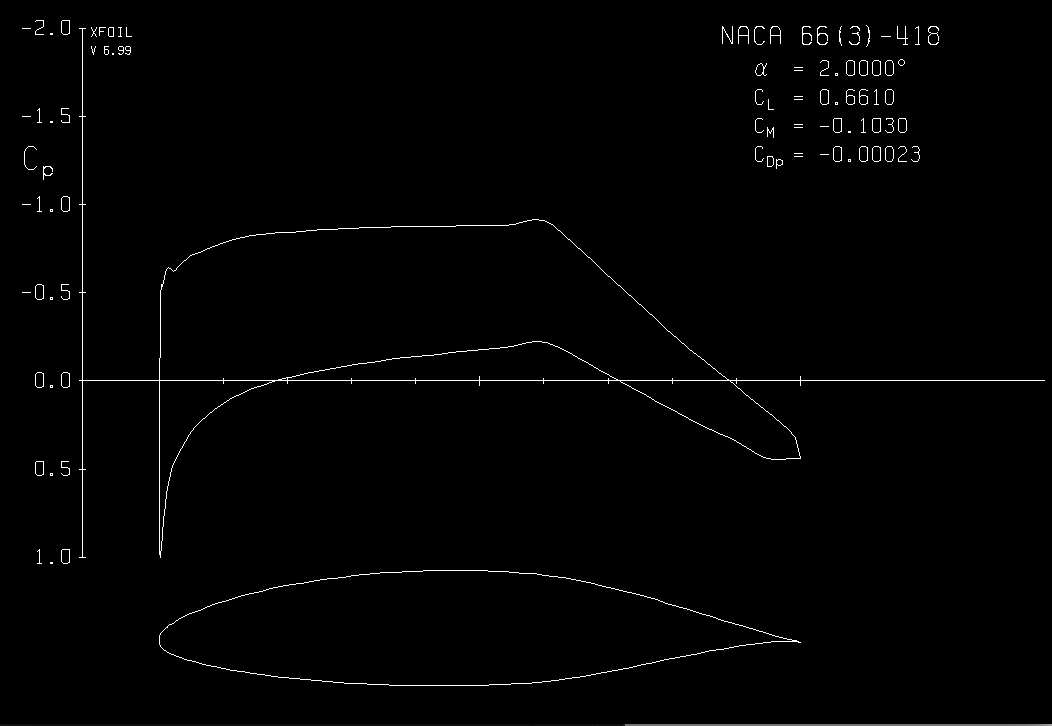
\includegraphics[width=0.55\textwidth]{parte4/cp}
    \caption{Coeficiente de pressão para o perfil da asa em condição de cruzeiro.}
\end{figure}

O $C_p$ mínimo desenvolvido é de $-0,91344$. Como o valor de $C_p$ é dado por
\begin{equation}
    C_p = 1 - \left(\frac{u}{u_\infty}\right)^2
\end{equation}
A velocidade máxima sobre o perfil é de $194\si{m/s}$, o que equivale a Mach $0,64$ a 30000ft. Esse valor é suficientemente baixo para afastar qualquer suspeita de escoamento transônico, e comprova que a seleção de perfil para a asa foi adequada